\documentclass[letterpaper]{article}

\usepackage{times}
\usepackage{helvet}
\usepackage{courier}
\usepackage[hyphens]{url}
\usepackage{graphicx}
\usepackage{booktabs}
\usepackage{amsmath}
\usepackage{amssymb}
\usepackage{listings}
\usepackage[hyphens]{url}
\urlstyle{rm}
\lstset{
  basicstyle={\small\ttfamily},
  breaklines=true,
  columns=fullflexible,
  keepspaces=true,
}

\title{Supplementary Appendix for\\
Consensus Is Not Completion: False Convergence in Multi-Agent Discovery Workflows}

\author{Anonymous Authors}

\begin{document}

\maketitle

\section{Purpose of the Appendix}

This appendix records experimental and implementation details that are useful
for reproducibility but are not required to follow the main argument. The main
paper is self-contained: it defines the problem, reports the principal results,
and states the limitations. The appendix expands the protocol, logging schema,
split rule, and audit-policy diagnostics.

\section{Closed-Loop Protocol}

Each experimental state follows the same loop:

\begin{enumerate}
    \item Fix a bounded source collection and oracle item set.
    \item Run discovery agents without shared intermediate answers, or run
    deterministic diagnostic scanners.
    \item Aggregate agent reports using consensus, standard summarization, raw
    union, or union-preserving summarization.
    \item Compute pre-audit observable signals from reports and metadata only.
    \item Apply the completion certificate without oracle labels or holdout
    gain.
    \item If required, run an audit policy over singleton, boundary, or
    source-partitioned evidence.
    \item Score final recall, precision, false-certification rate, audit
    recovery, and cost proxies against the oracle.
\end{enumerate}

\section{Evidence-Preserving Audit Policy Listing}

The main paper describes the audit controller; the procedural listing is:

\begin{enumerate}
    \item Run $k$ discovery agents without shared intermediate answers,
    producing $Y_1,\ldots,Y_k$.
    \item Compute item counts $n(y)=|\{i:y\in Y_i\}|$.
    \item Set conservative final set $F=\{y:n(y)\ge2\}$ and audit queue
    $Q=\{y:n(y)=1\}$.
    \item Compute pre-audit confidence, overlap, source coverage, and
    unseen-mass signals.
    \item Apply the pre-audit completion certificate.
    \item If the certificate is \textsc{safe-to-stop}, return $F$ with the
    certificate report.
    \item If $Q$ is non-empty, trigger singleton audit.
    \item If confidence and overlap are high and the task has
    boundary-resolution risk, trigger boundary-focused holdout audit.
    \item Add audit-verified singletons and holdout-discovered boundary items
    to $F$.
    \item Recompute the post-audit certificate using the updated ledger and
    return $F$ plus pre/post certificate reports.
\end{enumerate}

\section{Task Families and Oracles}

\begin{table}[h]
\centering
\small
\begin{tabular}{llrl}
\toprule
Task & Source type & Oracle size & Main role \\
\midrule
T1 & synthetic code repository & 35 & aggregation-loss controls \\
T2 & synthetic policy documents & 30 & blind-spot controls \\
T3 & Click repository snapshot & 149 & real-repo deprecation audit \\
T4 & Requests repository snapshot & 304 & real-repo TLS audit \\
T5 & itsdangerous repository snapshot & 160 & external timed-signing audit \\
\bottomrule
\end{tabular}
\caption{Task families used by the current paper.}
\end{table}

\section{Oracle Construction Protocol}

Each task uses a bounded source snapshot and a released oracle file under
\path|experiments/false_convergence_pilot/results/|. Oracle labels are used only
for offline scoring, not during blind agent generation or pre-audit
certification.

\begin{table}[h]
\centering
\small
\begin{tabular}{llll}
\toprule
Task & Oracle file & Commit / source & Size \\
\midrule
T1 & \path|T1_hard_repo_oracle.json| & synthetic AcmePay repo & 35 \\
T2 & \path|T2_policy_docs_oracle.json| & synthetic policy docs & 30 \\
T3 & \path|T4_real_repo_click_deprecation_oracle.json| &
Click \texttt{8a1b1a3} & 149 \\
T4 & \path|T5_real_repo_requests_tls_oracle.json| &
Requests \texttt{1190afd} & 304 \\
T5 & \path|T6_real_repo_itsdangerous_timed_signing_oracle.json| &
itsdangerous \texttt{672971d} & 160 \\
\bottomrule
\end{tabular}
\caption{Oracle artifacts used for scoring.}
\end{table}

\paragraph{Inclusion criteria.}
T1 includes code, configuration, registry, fallback, and replay locations that
resolve to AcmePay v1. T2 includes policy cases whose state, flow, and service
resolution imply AcmePay v1 handling. T3 includes Click line-level items in the
deprecated API surface audit, including implementation, warning emission, help
formatting, validation guards, tests, bounded changelog entries, and direct user
documentation. T4 includes Requests line-level items for TLS verification,
CA-bundle resolution, client certificates, TLS/SSL error handling, tests, test
infrastructure, and direct user documentation. T5 includes itsdangerous
timestamped signing, max-age expiration, exception, serializer, test,
documentation, export, and changelog lines.

\paragraph{Exclusion criteria.}
We exclude broad file-level answers, incidental keyword mentions outside the
task boundary, unrelated uses of terms such as \texttt{verify}, and files
outside the bounded task snapshot. For T3--T5, oracle files include an
\texttt{oracle\_policy} field describing these boundaries.

\paragraph{Construction process.}
The current oracles were built from task definitions, keyword/static scans,
source inspection, and manual normalization to line-level items with evidence
spans and buckets where available. The current paper treats them as closed-world
evaluation artifacts, but we do not claim independent double annotation. Before
submission, the real-repository oracles should receive an independent second
pass that records reviewer, changed items, ambiguous cases, and final resolution
rules.

\section{v2 Diagnostic Logging Schema}

The v2 offline diagnostic writes a candidate/action log with the following
fields:

\begin{lstlisting}
run_id, repository, task_family, seed, agent_id, model,
prompt_variant, round_id, query_or_action, source_file,
source_region, candidate_item, first_seen_round, support_count,
confidence, token_input, token_output, tool_calls, wall_clock
\end{lstlisting}

The run generated 2,970 runs, 1,572,201 candidate/action rows, 2,340 pre-audit
states, 439 safe states, and 1,901 unsafe states. Oracle labels are used only
after candidate generation for residual missing mass, calibration, and
evaluation.

\section{Split Rule}

Train, calibration, and test splits are grouped by
$(\text{repository}, \text{task family}, \text{seed})$. No derived state from a
group crosses splits. The current split uses seeds 1--2 for training, seed 3
for calibration, and seeds 4--5 for test. This prevents near-duplicate states
from the same seed from appearing in both calibration and test.

\section{Audit Policy Diagnostics}

\begin{table}[h]
\centering
\small
\begin{tabular}{lrrrr}
\toprule
Policy & States & Pre recall & Post recall & Recovered TP \\
\midrule
no audit & 936 & .267 & .267 & 0 \\
boundary holdout & 936 & .267 & .283 & 2,596 \\
random holdout & 936 & .267 & .306 & 7,026 \\
risk-triggered audit & 936 & .267 & .535 & 51,548 \\
source-partitioned audit & 936 & .267 & .535 & 51,552 \\
always holdout & 936 & .267 & 1.000 & 121,869 \\
\bottomrule
\end{tabular}
\caption{v2 held-out audit-policy summary. The deterministic offline holdout is
a diagnostic stress test and should not be read as an online LLM audit result.}
\end{table}

\subsection{Source-Aware Audit Prototype}

The T3 certificate tells the workflow not to stop, but a practical system also
needs an audit policy that converts retained evidence into recovery. We evaluate
an offline source-aware audit prototype over G3/holdout candidates, using
deterministic task-policy predicates over source lines. This is an audit-policy
upper bound, not a blind LLM result. On T3, the raw candidate pools average
0.998 recall but only 0.660 precision. Source-aware filtering keeps the same
average recall and raises precision to 1.000; a bounded source sweep reaches
1.000 recall and 1.000 precision. On T4, candidate filtering reaches 0.849
recall and 1.000 precision, showing that precise audit is possible but search
coverage remains insufficient.

\subsection{Per-Seed Audit Behavior and Cost Proxy}

The audit policy exposes rather than hides uncertainty. In T1 seed01, it audits
and verifies 13 singleton true positives. In T2 seed01, it verifies 2 singleton
true positives. In T2 seed02/03, there are no singletons, but high agreement and
high confidence trigger boundary-focused holdout, recovering 2 new items in each
seed. In T1 seed02/03, the audit policy leaves 4 and 5 singleton items in the
audit queue and does not mark completion, avoiding raw union's false positives.
In T3 seed01, the evidence-preserving audit policy reaches 0.993 recall and
0.955 precision by auditing singleton evidence. In seed02 and seed03, however,
the available holdout scout is itself incomplete, so the audit policy recovers
only to 0.805 and 0.832 recall. The completion certificate catches this boundary:
for all three T3 seeds it returns \textsc{unsafe-to-stop}, triggered by low mean
confidence, singleton missing-mass signals, and Chao unseen-mass estimates.

Removing singleton audit leaves the aggregation-loss singletons in T1 seed01 and
T2 seed01 unrecovered. Removing the common-blind-spot trigger leaves T2
seed02/03 at 28/30 recall despite perfect G3 agreement. Removing holdout
converts hidden risk into a \textsc{requires-audit} state but cannot recover
missing items. Thus the two triggers correspond to distinct failure mechanisms,
and holdout is the mechanism that turns retained risk into verified recovery.

The offline audit-policy stress-test logs do not contain reliable token or
wall-clock accounting, so we report a proxy cost: audit queue size plus one unit
per triggered holdout. Under this proxy, T1 seed01 uses 14 audit actions to
recover 13 true positives, T2 seed01 uses 3 actions to recover 2 true positives,
and T2 seed02/03 use one holdout unit to recover 2 true positives each. In T1
seed02/03, the audit policy avoids the 4 and 5 false positives introduced by raw
union, but correctly refuses to certify completion without further audit.

\section{v2 Leakage and Generalization Audit}

The v2 audit reads the frozen offline diagnostic table and writes new outputs to
\path|experiments/false_convergence_pilot/v2_audit_outputs/|. The declared v2
feature set excludes oracle and label columns (\path|recall|,
\path|true_positive|, \path|residual_missing_mass|, and \path|unsafe|),
task/repository identifiers, split/seed identifiers, run ids, post-audit fields,
and cost columns. All audited rows are pre-audit states. A metadata-only
shortcut probe is reported separately and is not used as a valid method.

\begin{table}[h]
\centering
\small
\begin{tabular}{lrrr}
\toprule
Setting & AUROC & FCR & Safe coverage \\
\midrule
v2 in-distribution test & .999 & .017 & .966 \\
metadata-only probe & .988 & -- & .000 \\
leave-one Click & .591 & -- & .000 \\
leave-one policy docs & .546 & -- & .000 \\
leave-one Requests & .695 & -- & .000 \\
\bottomrule
\end{tabular}
\caption{Frozen v2 audit. Held-out repository/task-family validation fails to
certify any state under the calibration criterion.}
\end{table}

\section{Online Requests Audit-Controller Evaluation}

We ran the P0 Requests TLS online audit-controller loop using
\texttt{gpt-5.3-codex}, seeds 04--08, search budget 180, max 1200 lines per
file, and the fixed Requests commit from the main paper. Outputs are stored in
\path|experiments/false_convergence_pilot/online_audit_controller/T5_requests_tls/|.
The online suite contains 60 blind discovery calls and 45 audit calls: five
boundary-focused holdout agents plus 40 random/singleton candidate-verifier
agents. The audit-policy result manifest is stored at
\path|experiments/false_convergence_pilot/online_audit_controller/T5_requests_tls/audit_policy_eval/MANIFEST.json|.

\begin{table}[h]
\centering
\small
\begin{tabular}{lrrrrrr}
\toprule
Condition & N & Jaccard & Consensus R & Union R & Precision & Tokens \\
\midrule
homogeneous & 5 & .813 & .678 & .732 & .710 & 213k \\
prompt-diverse & 5 & .778 & .662 & .724 & .709 & 213k \\
source-partitioned & 5 & .000 & .000 & .724 & .737 & 74k \\
independent-context & 5 & .285 & .626 & .732 & .729 & 143k \\
\bottomrule
\end{tabular}
\caption{Online discovery grid before post-audit evaluation. Source partitioning
keeps union recall comparable but makes vote-only consensus unusable.}
\end{table}

\begin{table}[h]
\centering
\small
\begin{tabular}{lrrrrrr}
\toprule
Policy & Pre R & Post R & Precision & Rec. TP & Intro. FP & Tokens \\
\midrule
no audit & .491 & .491 & .829 & 0.0 & 0.0 & 0k \\
random holdout & .491 & .554 & .755 & 18.9 & 11.9 & 17k \\
singleton audit & .491 & .719 & .725 & 69.1 & 38.7 & 12k \\
boundary holdout & .491 & .694 & .755 & 61.7 & 24.6 & 71k \\
source-partitioned review & .491 & .733 & .730 & 73.3 & 38.5 & 55k \\
risk-triggered audit & .491 & .733 & .713 & 73.3 & 45.5 & 83k \\
always holdout & .491 & .753 & .706 & 79.5 & 51.1 & 163k \\
\bottomrule
\end{tabular}
\caption{Online audit-policy means over 20 seed/configuration states. Tokens are
additional audit tokens.}
\end{table}

The full per-seed/per-condition logs are stored in
\path|audit_policy_eval/ONLINE_AUDIT_POLICY_RESULTS.csv| and
\path|audit_policy_eval/ONLINE_AUDIT_POLICY_RESULTS.md|. Discovery-grid means are
stored in
\path|ONLINE_DISCOVERY_GRID_SUMMARY.csv| and
\path|ONLINE_DISCOVERY_GRID_SUMMARY.md|. These results close the Requests P0
method-effect loop, but they also show a remaining gap: even always-holdout
averages only .753 recall, so the current controller should continue searching
or auditing rather than certify completion.

\section{Held-Out Click Staged Controller}

After the Requests development experiment, we froze a staged controller:
conservative consensus, singleton verification, source-partitioned review when
singleton mass/source gaps remain, and abstention whenever escalation was needed.
We then evaluated it on held-out online Click runs with seeds 04--06 and three
discovery configurations. Outputs are stored in
\path|experiments/false_convergence_pilot/online_heldout_click_staged_controller/|.

\begin{table}[h]
\centering
\scriptsize
\resizebox{\linewidth}{!}{
\begin{tabular}{lrrrrrrrr}
\toprule
Policy & Post R & Prec. & Rec. TP & Intro. FP & Audit tok. & E2E tok. & FCR & Abstain \\
\midrule
no audit & .465 & .769 & 0.0 & 0.0 & 0k & 166k & .000 & 1.000 \\
singleton audit & .722 & .630 & 38.2 & 29.6 & 9k & 175k & .000 & 1.000 \\
source-partitioned review & .755 & .577 & 43.2 & 44.8 & 57k & 223k & .000 & 1.000 \\
staged controller & .761 & .555 & 44.0 & 54.1 & 56k & 223k & .000 & 1.000 \\
always holdout & .768 & .492 & 45.1 & 80.3 & 177k & 343k & .000 & 1.000 \\
\bottomrule
\end{tabular}}
\caption{Held-out Click online results over nine seed/configuration states.
The staged controller nearly matches always-holdout recall at about one third of
the audit-token cost, but abstains on every state. Safe coverage is therefore
0.000, while false certification is also 0.000.}
\end{table}

These held-out results support a narrower claim than automatic completion: the
staged controller improves recall--cost tradeoff while preserving abstention
when source escalation is required. It does not yet solve safe-to-stop coverage.

\section{External itsdangerous Staged Controller}

The external validation repository is \texttt{pallets/itsdangerous} at commit
\texttt{672971d66a2ef9f85151e53283113f33d642dabd}. The staged controller,
prompt, budget, and thresholds were frozen before this task was scored. Outputs
are stored in
\path|experiments/false_convergence_pilot/online_external_itsdangerous_staged_controller/|.

\begin{table}[h]
\centering
\scriptsize
\resizebox{\linewidth}{!}{
\begin{tabular}{lrrrrrrrr}
\toprule
Policy & Post R & Prec. & F1 & Rec. TP & Intro. FP & Audit tok. & E2E tok. & Abstain \\
\midrule
no audit & .569 & .841 & .679 & 0.0 & 0.0 & 0k & 31k & 1.000 \\
singleton audit & .867 & .719 & .786 & 47.8 & 26.1 & 9k & 40k & 1.000 \\
source-partitioned review & .871 & .733 & .796 & 48.3 & 22.1 & 11k & 43k & 1.000 \\
staged controller & .879 & .709 & .785 & 49.7 & 29.6 & 19k & 50k & .889 \\
always holdout & .890 & .675 & .768 & 51.4 & 39.9 & 41k & 72k & 1.000 \\
\bottomrule
\end{tabular}}
\caption{External itsdangerous online results over nine seed/configuration
states. The staged controller has one certified unsafe state, so its
false-certification rate among certified states is 1.000 and safe coverage is
0.000.}
\end{table}

The safe-state sweep on seed04 added three boundary-focused agents with a larger
search budget. The base union had recall .894 and precision .641. The
boundary-augmented union had recall .900 and precision .634, recovering one
true positive and introducing three false positives at 39,602 additional audit
tokens. The sweep therefore did not produce a real online safe state.

\section{Bootstrap and Paired Tests}

The script
\path|experiments/false_convergence_pilot/tools/analyze_staged_controller_stats.py|
computes seed-clustered bootstrap intervals over Requests, Click, and
itsdangerous. Requests is included in policy means but excluded from staged
paired tests because the Requests development run did not include a frozen
staged-controller arm.

\begin{table}[h]
\centering
\scriptsize
\resizebox{\linewidth}{!}{
\begin{tabular}{lrrrr}
\toprule
Comparator & Recall diff & Precision diff & F1 diff & Audit-token diff \\
\midrule
singleton audit & .025 [.012,.039] & -.042 [-.067,-.019] & -.013 [-.025,-.002] & 28k [12k,47k] \\
source review & .007 [.005,.009] & -.023 [-.029,-.017] & -.012 [-.017,-.009] & 3k [-6k,9k] \\
always holdout & -.009 [-.013,-.005] & .048 [.034,.063] & .029 [.018,.039] & -71k [-111k,-37k] \\
\bottomrule
\end{tabular}}
\caption{Paired staged-controller differences over Click and itsdangerous. The
intervals are descriptive seed-clustered bootstrap 95\% intervals and should not
be used to retune the frozen controller.}
\end{table}

\section{Oracle Review and Replication Status}

The real-repository oracle review status is logged at
\path|experiments/false_convergence_pilot/oracle_reviews/ORACLE_SECOND_REVIEW_STATUS.md|.
No independent human second-review diff has been produced yet, so the paper
does not claim double annotation. Second-model replication is also not yet run;
it remains a TODO until a second model, fixed prompt, manifest, logs, and scores
are present.

\section{SeekerGym Status}

The SeekerGym local checkout/schema is not present, so no benchmark result is
claimed. The manifest is stored at
\path|experiments/false_convergence_pilot/benchmark_runs/seekergym/MANIFEST.json| and
contains only TODOs for schema mapping, oracle construction, trace conversion,
and cost logging.

TRQA and WideSearch are likewise not run in this repository. They should remain
TODO entries until a fixed subset, oracle mapping, run manifest, logs, and
scoring outputs exist.

\section{Additional Figures}

\begin{figure}[h]
\centering
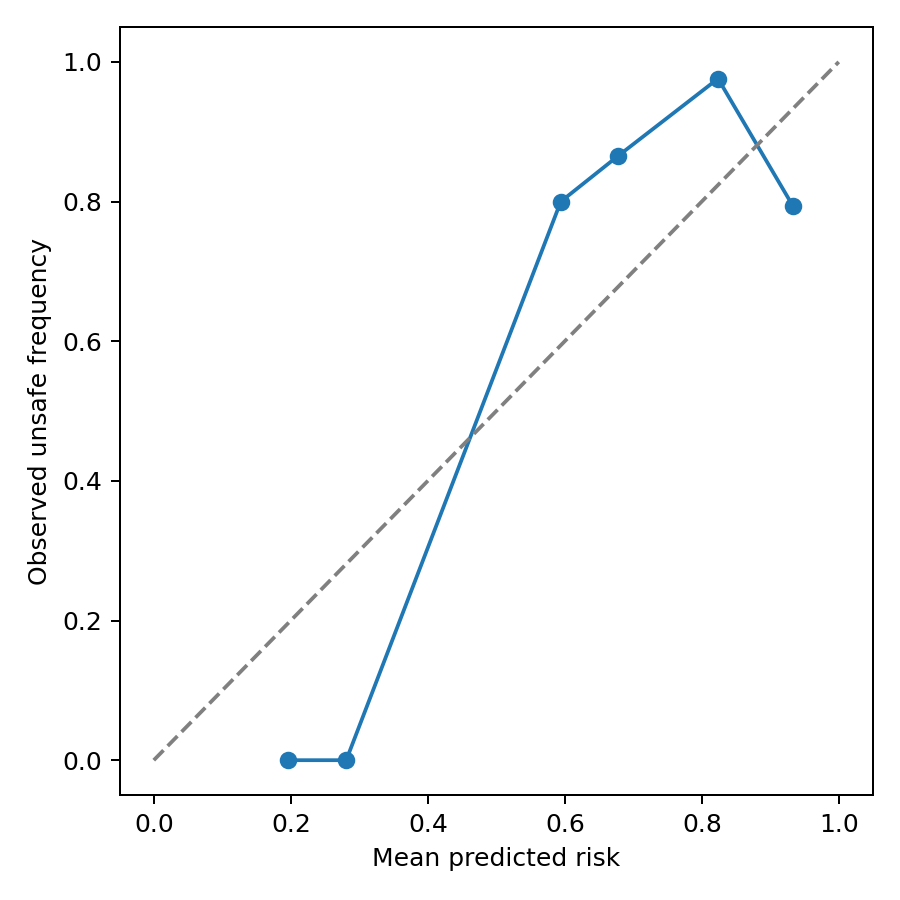
\includegraphics[width=.8\linewidth]{../../experiments/false_convergence_pilot/v2_outputs/figures/v2_calibration_curve_v1_proxy.png}
\caption{Calibration curve for the v1 risk proxy in the v2 diagnostic suite.}
\end{figure}

\end{document}
